\documentclass[10pt]{report}

\usepackage{stan-talks}

\begin{document}

\sf
\vspace*{6pt}
\noindent
\spc{\huge\bfseries \color{MidnightBlue}{Section 5.}
\\[8pt]
\spc{\Huge\bfseries \color{MidnightBlue}{Stan for ``Big Data''}}}
\vfill
\noindent
\spc{\large\bfseries Bob Carpenter}
\\[4pt]
\spc{Columbia University}
\vfill
\hfill 

\mypart{Part I}{Overview}

\sld{Scaling and Evaluation}
\begin{center}
\vspace*{-6pt}
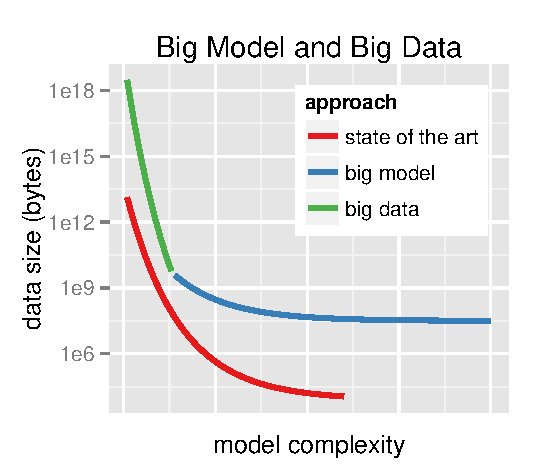
\includegraphics[width=0.6\textwidth]{img/big-model-big-data.pdf}
\vspace*{-6pt}
\end{center}
\begin{itemize}
\item Types of Scaling: data, parameters, \myemph{models}
\end{itemize}

\sld{Riemannian Manifold HMC}
\begin{itemize}
\item Best mixing MCMC method (fixed \# of continuous params)
\item Moves on Riemannian manifold rather than Euclidean
\begin{subitemize}
\item adapts to position-dependent curvature
\end{subitemize}
\item \myemph{geoNUTS} generalizes NUTS to RHMC (Betancourt {\slshape arXiv})
\item \myemph{SoftAbs} metric (Betancourt {\slshape arXiv})
\begin{subsubitemize}
\vspace*{-4pt}
\item eigendecompose Hessian and condition
\item computationally feasible alternative to original Fisher info metric
   of Girolami and Calderhead ({\slshape JRSS, Series B})
\item requires third-order derivatives and implicit integrator
\end{subsubitemize}
\vfill
\item Code complete; awaiting higher-order auto-diff
\end{itemize}

\sld{Adiabatic Sampling}
\begin{itemize}
\item Physically motivated alternative to ``simulated''
  \myemph{annealing and tempering} (not really simulated!)
\item Supplies external \myemph{heat bath}
\item Operates through \myemph{contact manifold}
\item System relaxes more naturally between energy levels
\item Betancourt paper on {\slshape arXiv}
  \vfill
\item Prototype complete
\end{itemize}


\sld{``Black Box'' Variational Inference}
\begin{itemize}
%
\item \myemph{Black box} so can fit any Stan model
%
\item Multivariate \myemph{normal approx to unconstrained} posterior
\begin{subitemize}
\item covariance: diagonal mean-field or full rank
\item not Laplace approx --- around posterior mean, not mode
\item transformed back to constrained space (built-in Jacobians)
\end{subitemize}
%
\item Stochastic \myemph{gradient-descent} optimization
\begin{subitemize}
\item ELBO gradient estimated via Monte Carlo + autdiff
\end{subitemize}
%
\item Returns \myemph{approximate posterior} mean / covariance
\item Returns \myemph{sample} transformed to constrained space
\end{itemize}

\sld{``Black Box'' EP}
\begin{itemize}
\item Fast, approximate inference (like VB)
\begin{subitemize}
\item VB and EP minimize divergence in opposite directions
\item especially useful for Gaussian processes
\end{subitemize}
%
\item Asynchronous, data-parallel \myemph{expectation propagation}
  (EP)
\item Cavity distributions control subsample variance
%
\vfill
%
\item Prototypte stage
\item {\small collaborating with Seth Flaxman, Aki Vehtari, Pasi
    Jyl\"anki, John Cunningham, Nicholas Chopin, Christian Robert}
\end{itemize}

\sld{The Cavity Distribution}
\vspace*{-6pt}
\begin{center}
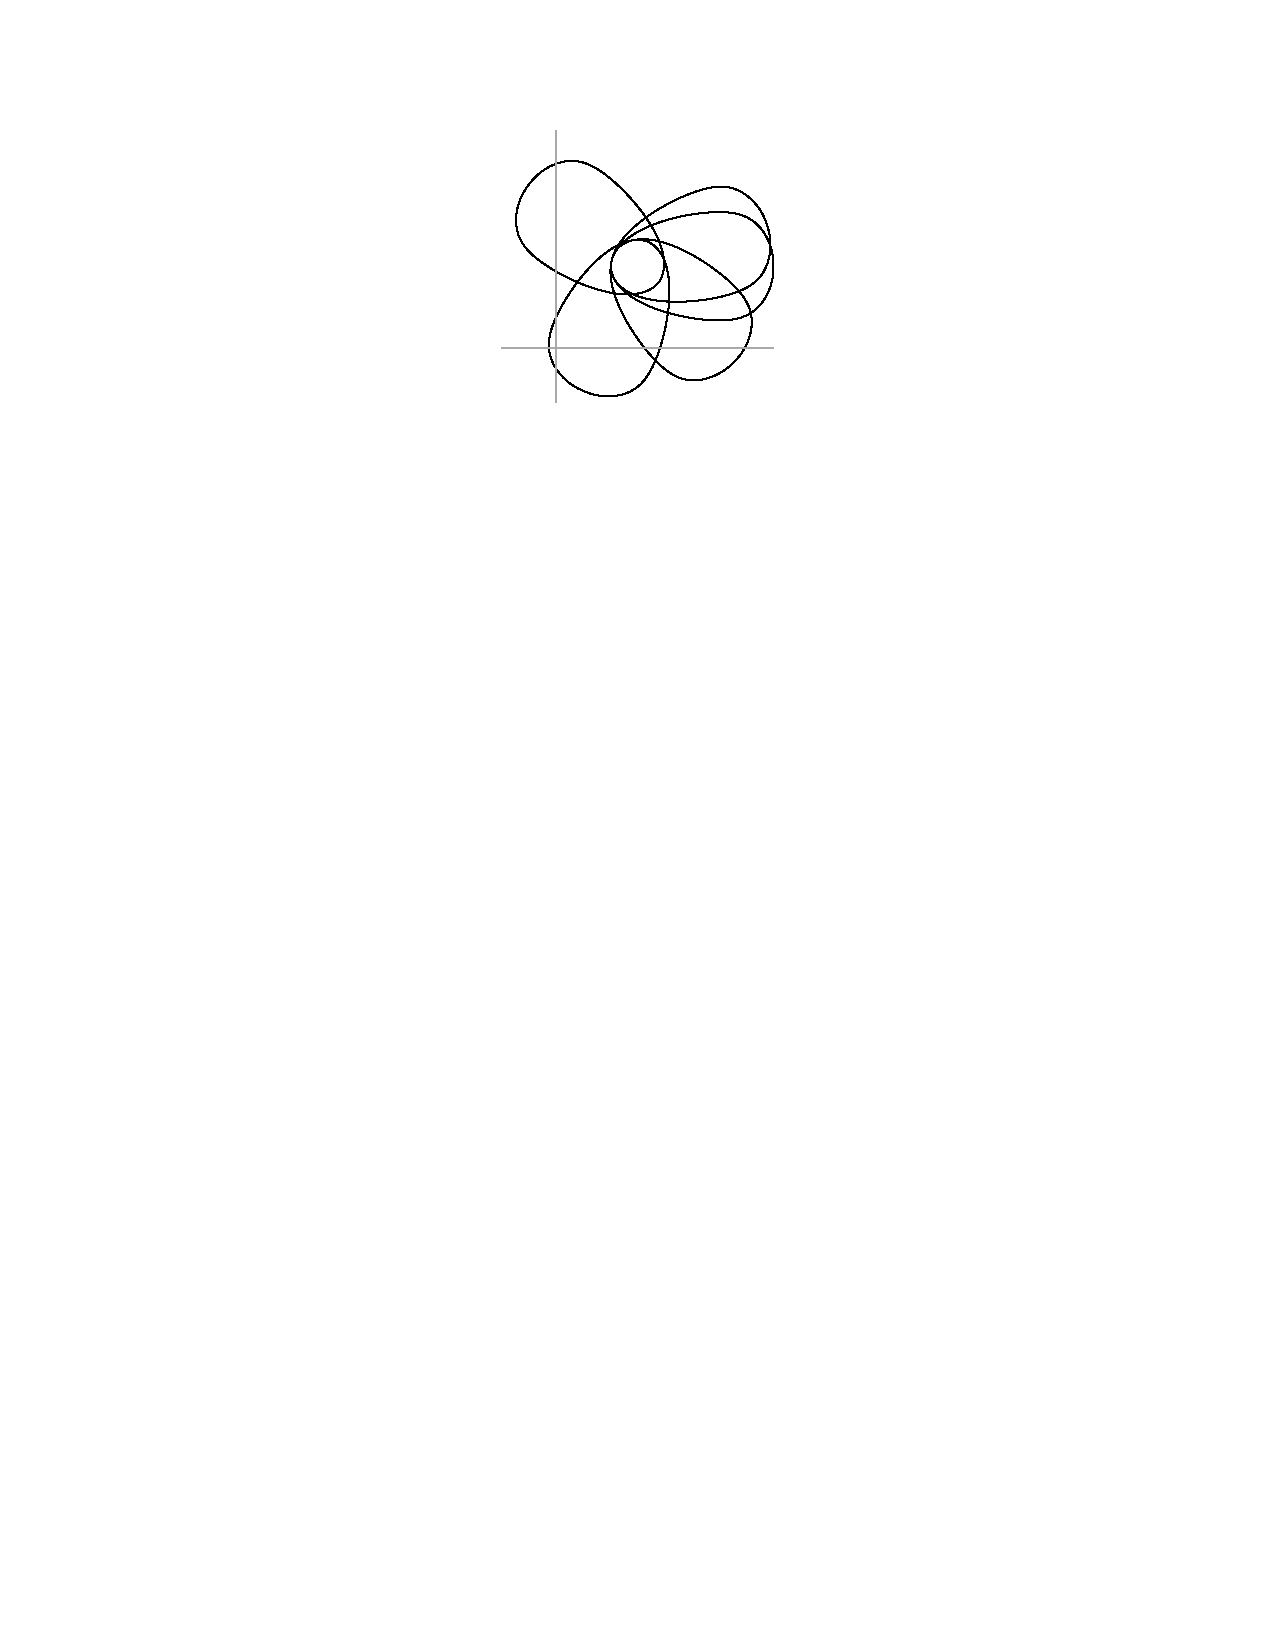
\includegraphics[width=0.25\textwidth]{img/ep-cavity.pdf}
\end{center}
\vspace*{-8pt}
\begin{subitemize}
\item Two parameters, with data split into $y_1, \ldots, y_5$
\item Contours of likelihood $p(y_k | \theta)$ for $k \in 1{:}5$
\item $g_{-k}(\theta)$ is \myemph{cavity distribution} (current
  approx. without $y_k$)
\item Separately computing for $y_k$ reqs each partition to cover its area
\item Combining likelihood with cavity \myemph{focuses on overlap}
\end{subitemize}

\sld{Maximum Marginal Likelihood}
\begin{itemize}
\item Fast, approximate inference for hierarchical models
\item Marginalize out lower-level parameters
\item Optimize higher-level parameters and fix
\item Optimize lower-level parameters given higher-level
\item Errors estimated as in MLE
\item aka ``empirical Bayes''
\begin{subitemize}
\item but not fully Bayesian
\item and no more empirical than full Bayes
\end{subitemize}
\item Design complete; awaiting parameter tagging
\end{itemize}


\mypart{Part II}{Posterior Modes \& \\[8pt] \spc Laplace Approximation}

\sld{Laplace Approximation}
\begin{itemize}
\item Multivariate normal approximation to posterior
\item Compute posterior mode via optimization
\[
\theta^{*} = \argmax_{\theta} \  p(\theta | y) 
\]
\item Laplace approximation to the posterior is
\[
p(\theta | y) 
\approx 
\distro{MultiNormal}(\theta^{*} | -H^{-1})
\]
\item $H$ is the Hessian of the log posterior
\[
H_{i,j} 
= \frac{\partial^2}{\partial \theta_i \ \partial \theta_j}
  \log p(\theta | y)
\]
\end{itemize}


\sld{Stan's Laplace Approximation}
\begin{itemize}
\item Operates on unconstrained parameters
\item L-BFGS to compute posterior mode $\theta^*$
\item Automatic differentiation to compute $H$
\begin{subitemize}
\item current R: finite differences of gradients
\item soon:  second-order automatic differentiation
\end{subitemize}
\item Draw a sample from approximate posterior
\begin{subitemize}
\item transfrom back to constrained scale
\item allows Monte Carlo computation of expectations
\end{subitemize}
\end{itemize}


\mypart{Part III}{Variational Bayes}

\sld{VB in a Nutshell}
\begin{itemize}
\item $y$ is observed data, $\theta$ parameters
\item Goal is to approximate posterior $p(\theta | y)$
\item with a convenient approximating density $g(\theta | \phi)$
\begin{subitemize}
\item $\phi$ is a vector of parameters of approximating density
\end{subitemize}
\item Given data $y$, VB computes $\phi^*$ 
minimizing KL-divergence
\begin{subitemize}
\item from approximation $g(\theta \, | \, \phi)$ to posterior $p(\theta \, | \, y)$
\end{subitemize}
\begin{eqnarray*}
\phi^* 
& = & 
\displaystyle
\argmin_\phi \ \mbox{KL}[g(\theta|\phi) \ || \ p(\theta|y)]
\\[4pt]
& = & 
\displaystyle
\argmax_\phi 
-\int_{\Theta} 
  \log\left(
    \frac{p(\theta \, | \, y)}{g(\theta \, | \, \phi)}
  \right)
  \ g(\theta | \phi) \ \mathrm{d}\theta
\end{eqnarray*}
\end{itemize}

\sld{VB vs.\ Laplace}
\vspace*{-6pt}
\begin{center}
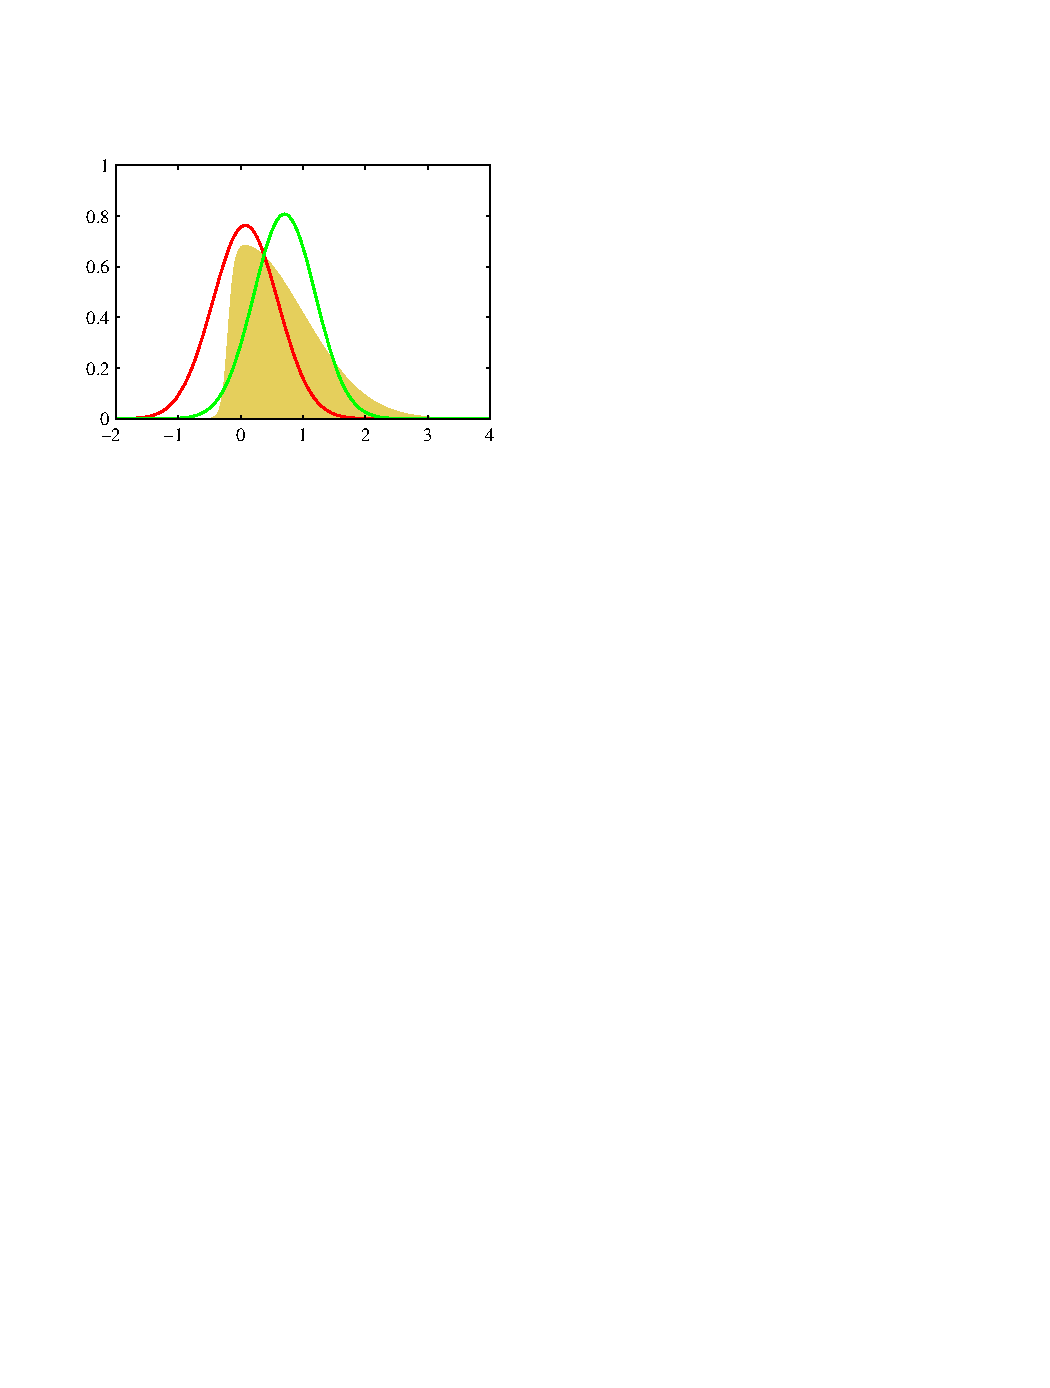
\includegraphics[width=0.45\textwidth]{img/bishop-fig-10-1.pdf}
\end{center}
\vspace*{-10pt}
\begin{itemize}
\item {\slshape solid yellow}: target; \ \ {\slshape red}: Laplace; \ \
  {\slshape green}: VB
\item \myemph{Laplace} located at posterior mode
\item \myemph{VB} located at approximate posterior mean
\end{itemize}
\vfill \hfill
{\footnotesize  --- Bishop (2006) {\slshape Pattern Recognition and Machine Learning}, fig.~10.1}

\sld{KL-Divergence Example}
\vspace*{-4pt}
\begin{center}
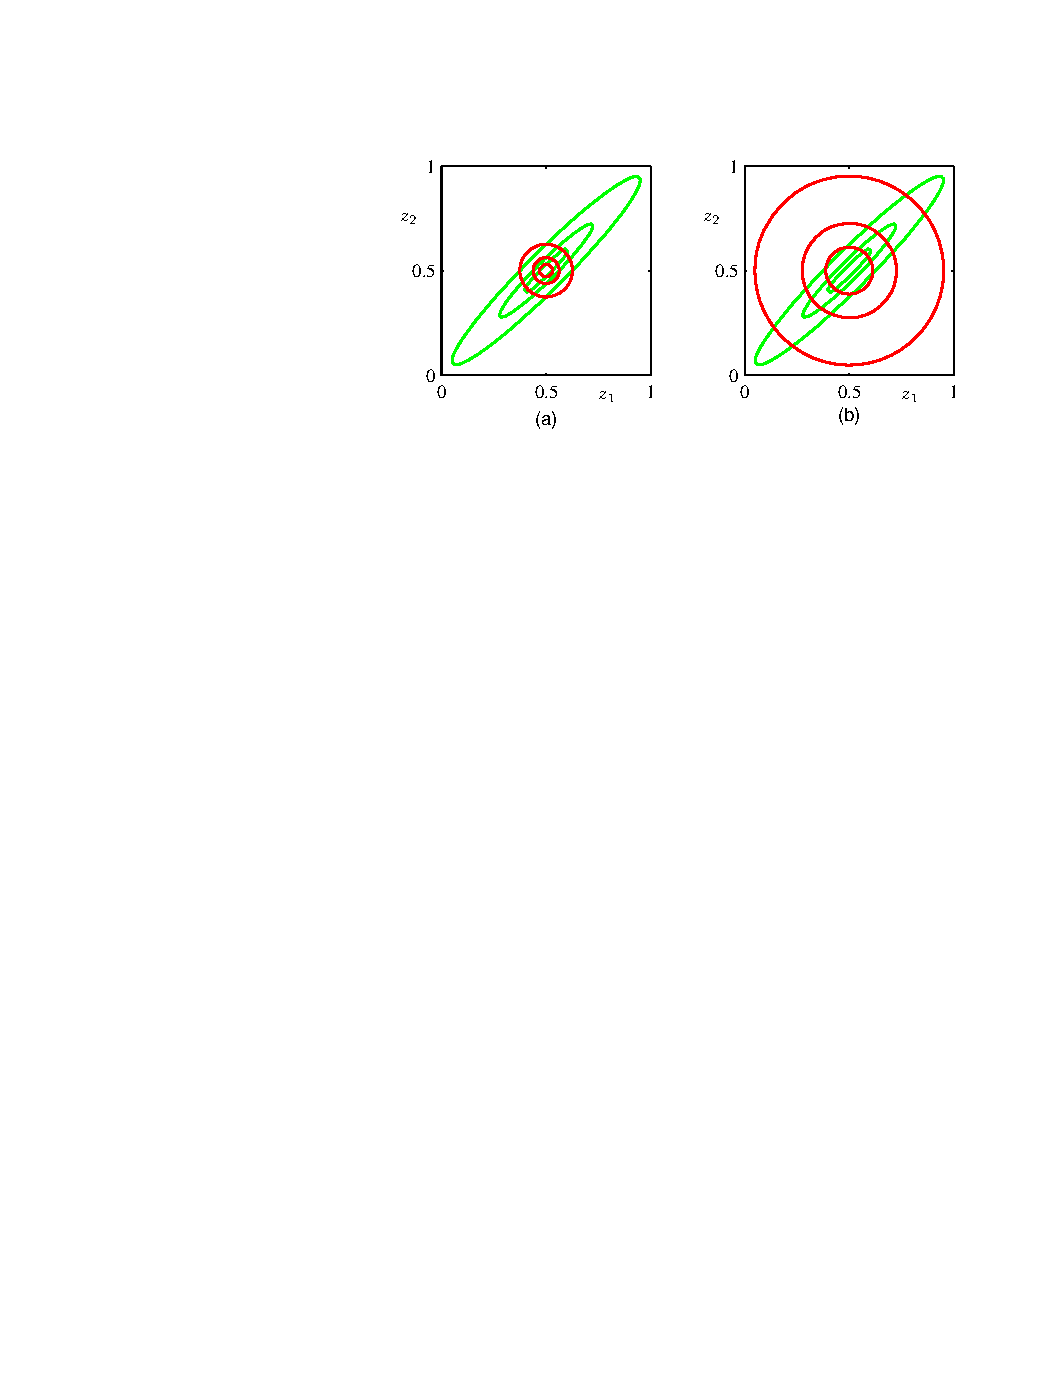
\includegraphics[width=0.6\textwidth]{img/bishop-fig-10-2.pdf}
\end{center}
\vspace*{-10pt}
\begin{subitemize}
\item \myemph{Green}: true distribution $p$; \ \ \myemph{Red}: best
  approximation $g$
\begin{subitemize}
\item[(a)] VB-like: $\mbox{KL}[g \, || \, p]$
\item[(b)] EP-like: $\mbox{KL}[p \, || \, g]$
\end{subitemize}
\item VB systematically \myemph{understimates posterior variance}
\end{subitemize}
\vfill \hfill
{\footnotesize  --- Bishop (2006) {\slshape Pattern Recognition and Machine Learning}, fig.~10.2}

\sld{Stan's ``Black-Box'' VB}
\begin{itemize}
\item Typically custom $g()$ per model
\begin{subitemize}
\item based on conjugacy and analytic updates
\end{subitemize}
\item Stan uses ``black-box VB'' with multivariate Gaussian $g$
\[
g(\theta|\phi) = \distro{MultiNormal}(\theta \, | \, \mu, \Sigma)
\]
for the \myemph{unconstrained posterior}
\begin{subitemize}
\item e.g., scales $\sigma$ log-transformed with Jacobian
\end{subitemize}
\item Stan provides two versions
\begin{subitemize}
\item Mean field: $\Sigma$ diagonal
\item General: $\Sigma$ dense
\end{subitemize}
\end{itemize}

\sld{Stan's VB: Computation}
\begin{itemize}
\item Use L-BFGS optimization to optimize $\theta^*$
\item Requires differentiable $\mathrm{KL}[g(\theta|\phi) \ || \ p(\theta|y)]$
\begin{subitemize}
\item only up to constant (i.e., use evidence lower bound (ELBO))
\end{subitemize}
\item Approximate KL-divergence and gradient via Monte Carlo
\begin{subitemize}
\item KL divergence is an expectation w.r.t. approximation $g(\theta|\phi)$
\item Monte Carlo draws i.i.d.\ from approximating multi-normal
\item only need approximate gradient calculation for soundness
\item so only a few Monte Carlo iterations are enough
\end{subitemize}
\end{itemize}

\sld{Stan's VB: Computation (cont.)}
\begin{itemize}
\item To support compatible plug-in inference
\begin{subitemize}
\item draw Monte Carlo sample $\theta^{(1)}, \ldots, \theta^{(M)}$ with
\[
\theta^{(m)} \sim  \distro{MultiNormal}(\theta \, | \, \mu^{*}, \Sigma^{*})
\]
\item inverse transfrom from unconstrained to constrained scale
\item report to user in same way as MCMC draws
\vfill
\end{subitemize}
\item Future: reweight $\theta^{(m)}$ via importance sampling
\begin{subitemize}
\item with respect to true posterior
\item to improve expectation calculations
\end{subitemize}
\end{itemize}

\sld{Near Future: Stochastic VB}
\begin{itemize}
\item Data-streaming form of VB 
\begin{subitemize}
\item Scales to billions of observations
\item {\footnotesize Hoffman et al. (2013) Stochastic variational inference. {\slshape JMLR} 14.}
\end{subitemize}
\item Mashup of stochastic gradient (Robbins and Monro 1951) and VB
\begin{subitemize}
\item subsample data (e.g., stream in minibatches)
\item upweight each minibatch to full data set size
\item use to make unbiased estimate of true gradient
\item take gradient step to minimimize KL-divergence
\end{subitemize}
\vfill
\item Prototype code complete
\end{itemize}


\mypart{}{The End (Section 5)}

\end{document}
